%!TEX root = ../Thesis.tex
\chapter{Simulations of Transfer Orbits} \label{ch:simulations-of-transfer orbits}
\epigraph{``\itshape{If you don’t put your breaks on when you reach the moon with a spaceship with people in it, you just keep going. And you’re dead. So the Hohmann transfer is risky, it’s a little bit dangerous and it uses a lot of fuel because you have to slow down (…). I think Apollo used a couple hundred pounds of fuel to slow down. It’s a million dollars a pound to bring anything to the Moon, including fuel. So just to slow down was a quarter of a billion dollars. I’m thinking, can you go into orbit without using your engines? Then you save all that money.}"}{--- \textup{Edward Belbruno}, Painting the Way to the Moon (2015)}


%%%%%%%%%%%%%%%%%%%%%%%%%%%%%%%%%%%%%%%%%%%%%%%%%%%%%%%%%%%%%%%%%%%%%%%%%%%%%%
\section{Setup and Circular Orbits}
Our search algorithm is basically a brute force search. All orbits are found by search method that start from circular Earth Orbit 160 km altitude to circular Moon Orbit 100 km altitude.

A search algorithm in our program then initiates many trajectory calculations with many slightly different initial conditions in the following manner:
\begin{enumerate}
    \item Many different initial positions in Earth parking orbit denoted by $\theta$, the angle from the positive $x$ axis, see figure \ref{fig:r3b} for reference. 
    \item Many $\Delta v_{\text{earth}}$ around some value.
    \item Many small variations of $\Delta \phi$, the angle between impulse $\vec{\Delta v}$ and start velocity vector $\vec{v_0}$.
\end{enumerate}

Each of the trajectories are iteratively calculated using the adaptive Verlet algorithm described in chapter \ref{ch:numerical-analysis} with the additional conditions:
\begin{enumerate}
    \item If we hit the earth, the trajectory is discarded.
    \item If we hit the moon at altitude $\SI[separate-uncertainty=true]{100(10)}{\km}$, the necessary $\Delta v_{\text{moon}}$ to enter circular orbit is calculated and applied.
\end{enumerate}
Throughout a simulation run, only the trajectory with the lowest $\Delta v_{\text{moon}}$ is saved. This effectively filters out all the trajectories hitting the Moon head-on or high velocities; the best orbit will enter the Moon's orbit on an angle approximately tangent to a $\SI{100}{\km}$ circular orbit.


%%%%%%%%%%%%%%%%%%%%%%%%%%%%%%%%%%%%%%%%%%%%%%%%%%%%%%%%%%%%%%%%%%%%%%%%%%%%%%
\section{Hohmann Transfer Orbits}
If the moon was stationary in an inertial system, we would simply shoot from the opposite side of the Earth, at $\theta = \pi$. But because we must shoot not for where the moon is, but for where the moon will be. We also know that the flight time is approximately $5$ days. We search for Hohmann orbits with simulation times of 6 days as follows:
\begin{enumerate}
    \item Angular position from Earth varied in 100 positions uniformly spaced around $\theta=-3\pi/4$ in range $\pm\ \pi/4.$
    \item Earth burn $\Delta v_{\text{earth}}$ varied in 200 velocities uniformly around $\SI{3.11}{\km\per\s}$ (found by trial-and-error, starting from \ref{eq:deltav-earth}) in range $\pm 0.1*\texttt{unit\_velocity} = \SI{0.102}{\km\per\s}.$
    \item One refinement-run on the best trajectory as initial guess, where all the ranges are set to 1/10 their previous value, and number of all three parameters set to 55.
\end{enumerate}

Listing \ref{lst:hohmann} show the lowest energy Hohmann trans-lunar injection found among $100 \times 200 + 55 \times 55 \times 55  = 20000 + 3375 = 23375$ trajectories.

%\begin{minipage}{\linewidth}
\begin{adjustwidth*}{0cm}{-0.4cm}
\begin{lstlisting}[caption={Best Hohmann orbit. \texttt{pos} = angular difference with start angle (here $\theta=-3\pi/4$), \texttt{ang} = angle to velocity vector in Earth parking orbit, \texttt{burn} = $\Delta v_{\text{earth}}$, \texttt{(x0,y0,px0,py0)} are the initial conditions.},label=lst:hohmann]
# --------------------------------------------------------------------------
duration = 5/unit_time
pos      = -2.086814820119193
ang      = -0.000122173047640
burn     = 3.111181716545691/unit_vel
x0       = -0.020532317163607
y0       = -0.014769797663479
px0      = 9.302400979050308
py0      = -5.289712560652044
# --------------------------------------------------------------------------
# dV(earth-escape) = 3.111182 km/s
# dV(moon-capture) = 0.800682 km/s
# dV(total)        = 3.911863 km/s
# Flight-time      = 4.300078 days
# --------------------------------------------------------------------------
# Runtime = 0.51s
# Final position: 0.992505 -0.001507
# Final impulse: 0.503920 2.476928
# Final H: -2.730124
# Total runtime = 0.67s
# --------------------------------------------------------------------------
\end{lstlisting}
\end{adjustwidth*}
%\end{minipage}

See figure \ref{fig:hohmann-position} - \ref{fig:hohmann-H} for trajectory position-, entry/exit- and Hamiltonian plots.

\begin{figure}[ht!]
    \centering
        \subbottom[Short LETO in co-rotating $(x,y)$, Earth and Moon stationary.]{
            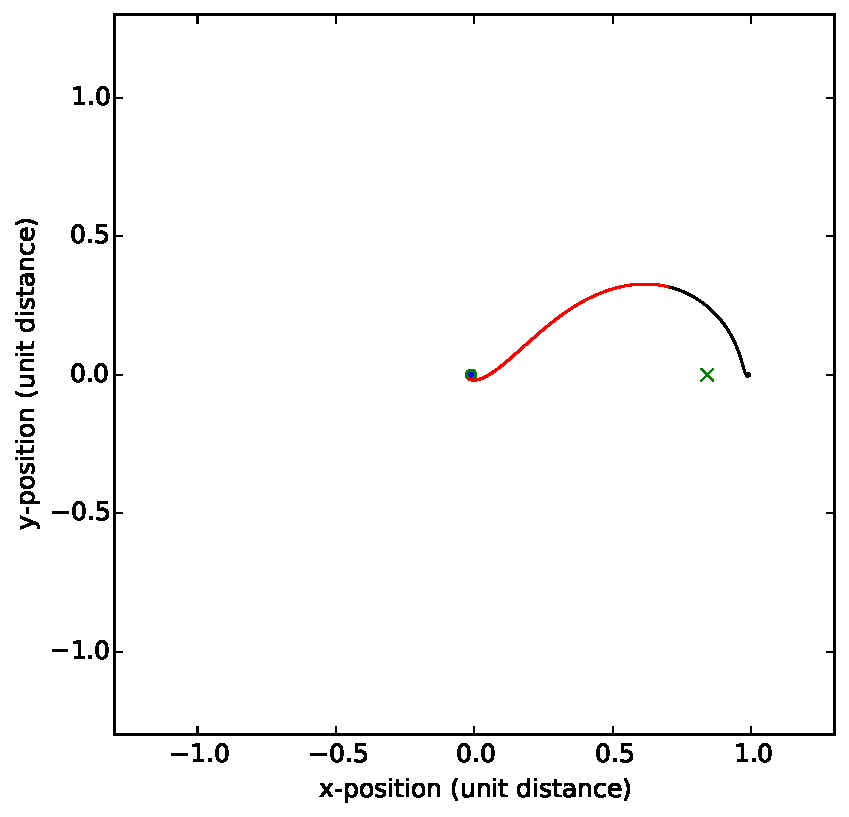
\includegraphics[scale=0.4]{fig/hohmann/_x-y_Hohmann.pdf}    
        }
        \subbottom[Hohmann in $(\mathscr{X},\mathscr{Y})$, inertial system stationary on CM.]{
            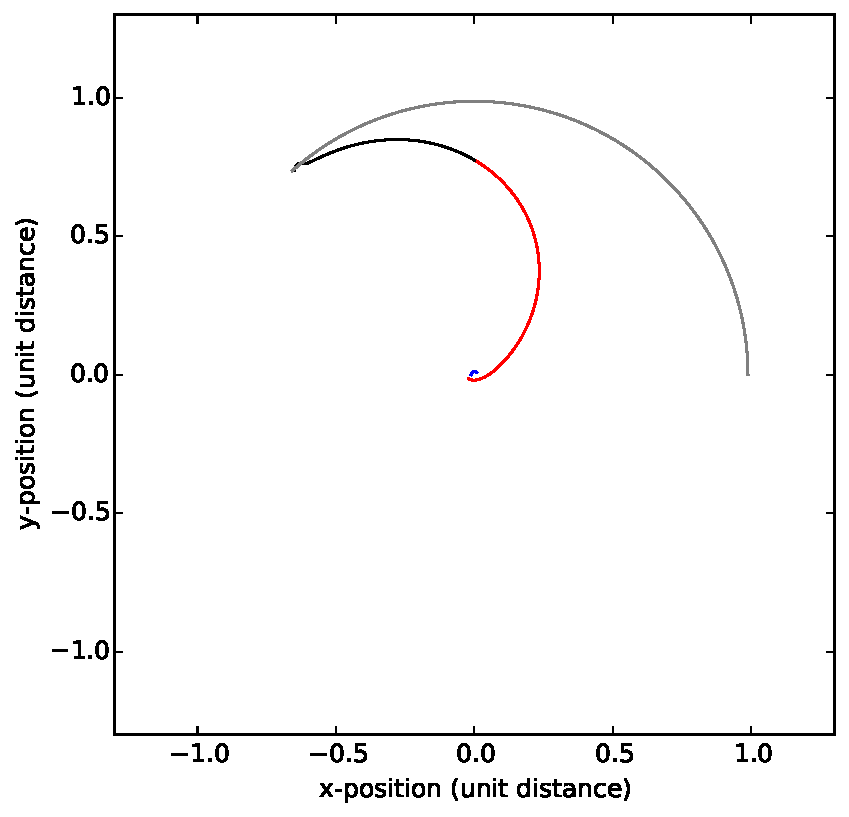
\includegraphics[scale=0.4]{fig/hohmann/X-Y_Hohmann.pdf}
        }
        \caption{Position plots of simulated Hohmann transfer-orbit. Earth in origin, moon orbit in grey, first half of trajectory is red, last half is black, green cross is first Lagrangepoint $L_1$}
        \label{fig:hohmann-position}
\end{figure}

\begin{figure}[ht!]
    \centering
        \subbottom[Exit from circular Earth parking orbit, $\SI{100}{\km}$ altitide]{
            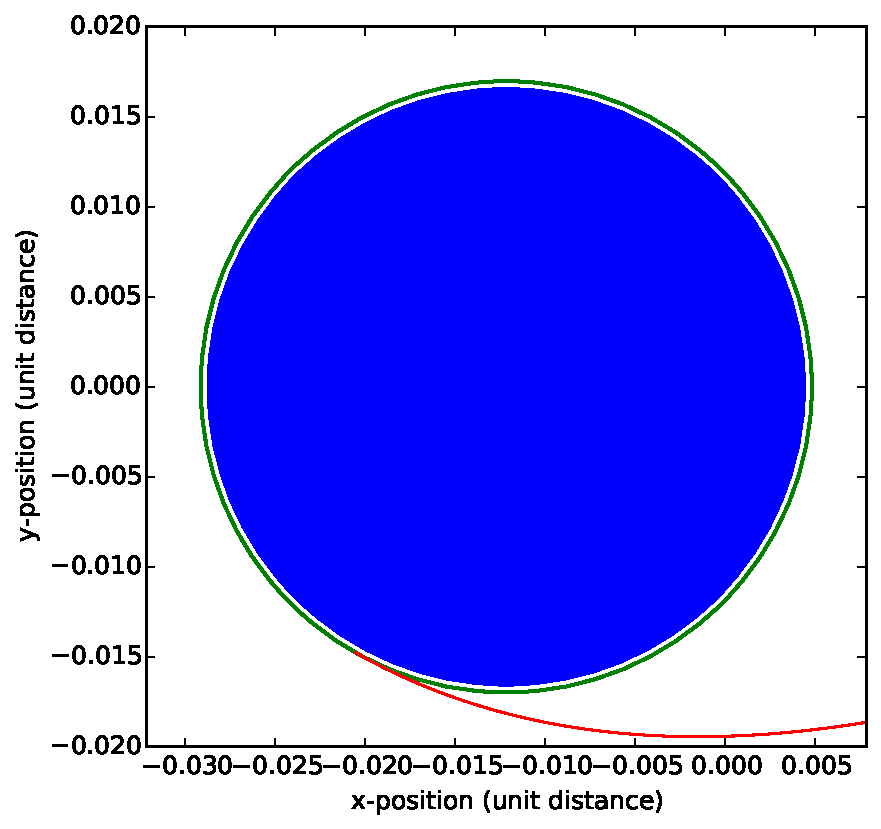
\includegraphics[scale=0.4]{fig/hohmann/earth_Hohmann.pdf}    
        }
        \subbottom[Entry to circular Moon orbit, $\SI{100}{\km}$ altitude]{
            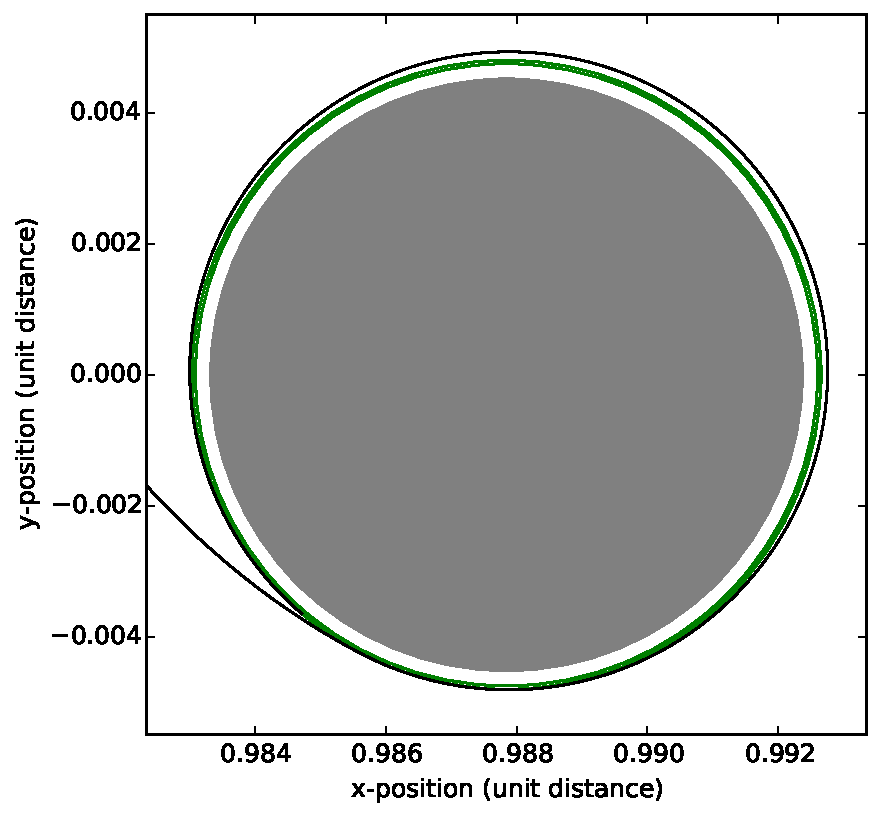
\includegraphics[scale=0.4]{fig/hohmann/moon_Hohmann.pdf}
        }
        \caption{Exit- and entry orbits of simulated Hohmann. The green band around the moon is the altitude range of \SI{\pm 10}{\km} around \SI{100}{\km} that triggers a capture, meaning a $\Delta v_{\text{moon}}$ is calculated and applied if a discrete time step lands inside this band}
        \label{fig:hohmann-exit_entry}
\end{figure}

\begin{figure}[ht!]
    \centering
        \subbottom[Step size.]{
            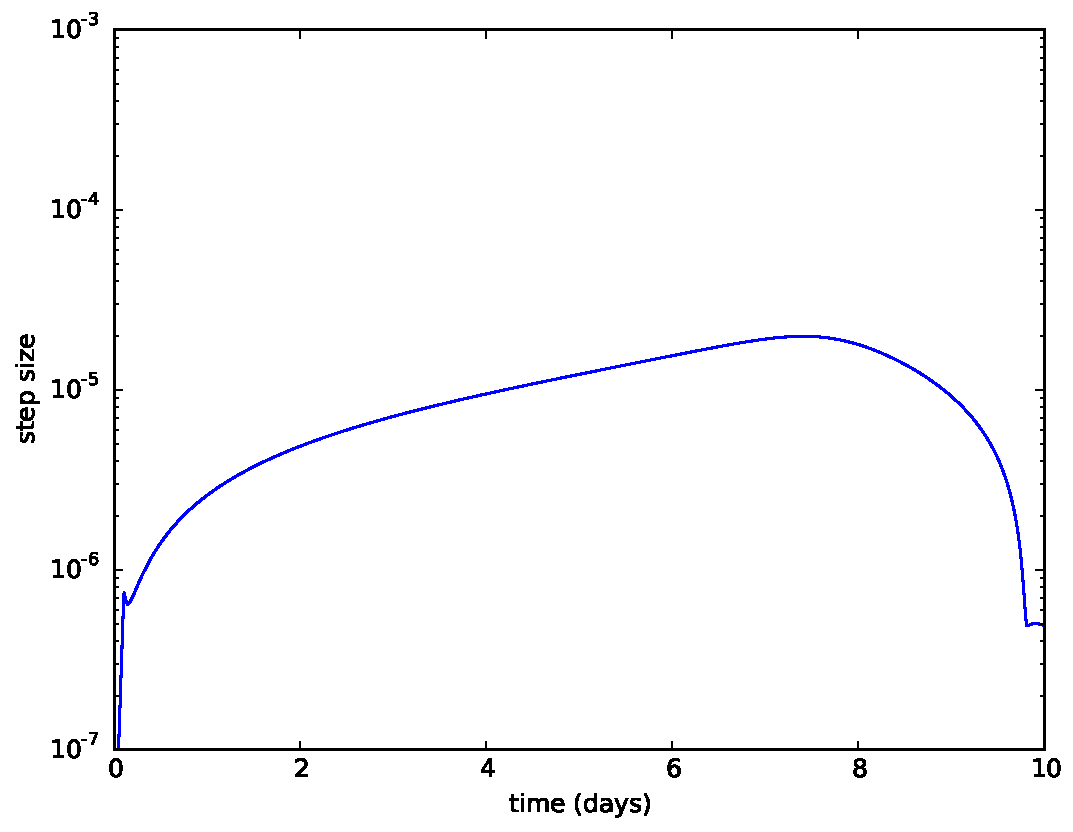
\includegraphics[scale=0.35]{fig/hohmann/step_Hohmann.pdf}    
        }
        \subbottom[Error per step.]{
            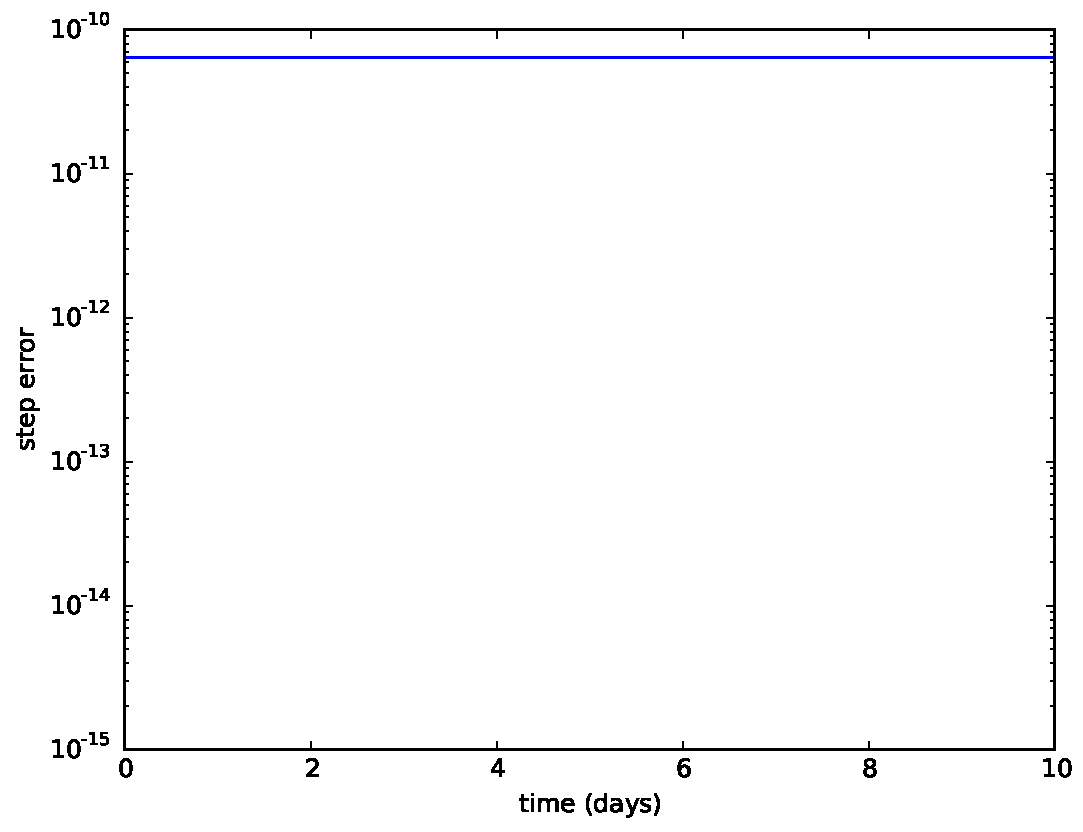
\includegraphics[scale=0.35]{fig/hohmann/err_Hohmann.pdf}
        }
        \caption{Step size and error per step of simulated Hohmann. As expected step size is longer in weaker gravitational field and vice versa, and constant in circular orbit. Error is maintained at $10^{-9}$, as ensured by the adaptive method}
        \label{fig:hohmann-step_error}
\end{figure}

\begin{figure}[ht!]
\centering
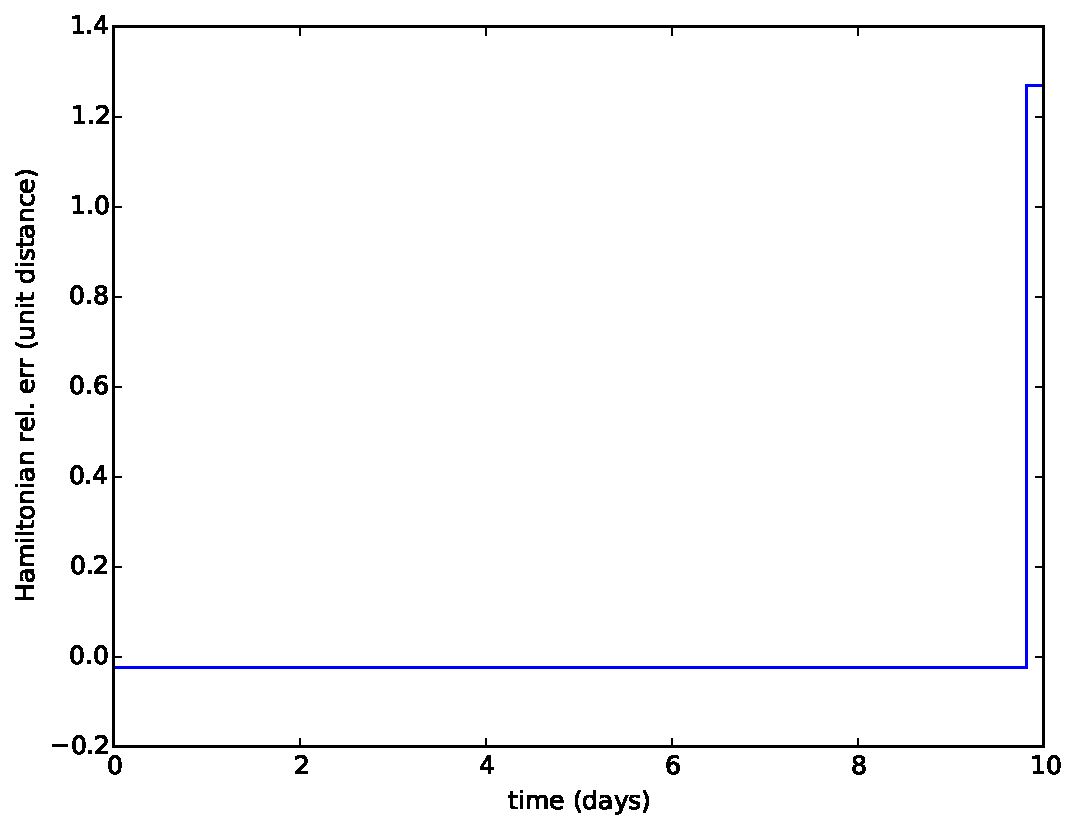
\includegraphics[scale=0.35]{fig/hohmann/H_Hohmann.pdf}
\caption{Hamiltonian $H$ is conserved along the trajectory until $\Delta v_{\text{moon}}$ is applied, as expected}
\label{fig:hohmann-H}
\end{figure}
Note from listing \ref{lst:hohmann} that $\Delta v_{\text{total}} = \SI{3.911}{\km}$ is in within reasonable agreement with the prediction from the simple Hohmann model in chapter \ref{ch:transfer orbits} of $\Delta v_{\text{total}} = \SI{3.946}{\km}$. Now we just need to see if we can find a low-energy transfer-orbit significantly cheaper than this.


%%%%%%%%%%%%%%%%%%%%%%%%%%%%%%%%%%%%%%%%%%%%%%%%%%%%%%%%%%%%%%%%%%%%%%%%%%%%%%
\section{Low-Energy Transfer Orbits (LETO)}
We searched for LETOs running simulations up to 200 days as follows:
\begin{enumerate}
    \item Angular position from Earth varied in 55 positions uniformly spaced around $\theta=0$ in range $\pm\ \pi$, i.e. in all directions.
    \item Earth burn $\Delta v_{\text{earth}}$ varied in 55 velocities uniformly around $\SI{3.12}{\km\per\s}$ (found by trial-and-error) in range $\pm 0.1*\texttt{unit\_velocity} = \SI{0.102}{\km\per\s}.$
    \item Angle $\phi$ to velocity vector in circular orbit varied in 55 angles uniformly spaced around $\phi=0$ in range $\pm \pi/100.$
    \item 7 refinement-runs around the iteratively best trajectory, where all the ranges are set to 1/10 their previous value.
\end{enumerate}

We will look at two LETOs:
\begin{description}
    \item[Short LETO] Flight time of 40.6 days and $\Delta_v{\text{total}} = \SI{3.896}{\km\per\s}$, found in simulation run with maximum duration of 41 days.
    \item[Long LETO] Flight time of 194.3 days and $\Delta_v{\text{total}} = \SI{3.795}{\km\per\s}$, found in a simulation run of 195 days.
\end{description}
Both was found with the same search parameters, except simulation duration among $55 \times 55 \times 55 \times 8 =$ 1,331,000 trajectories as described above.


%%%%%%%%%%%%%%%%%%%%%%%%%%%%%%%%%%%%%%%%%%%%%%%%%%%%%%%%%%%%%%%%%%%%%%%%%%%%%%
\subsection{Short LETO}
Listing \ref{lst:low_energy_short} show the lowest $\Delta v_{\text{total}}$ LETO trans-lunar injection 

%\begin{minipage}{\linewidth}
\begin{adjustwidth*}{0cm}{-0.4cm}
\begin{lstlisting}[caption={Short LETO. \texttt{pos} = angular difference with start angle (here $\theta=-3\pi/4$), \texttt{ang} = angle to velocity vector in Earth parking orbit, \texttt{burn} = $\Delta v_{\text{earth}}$, \texttt{(x0,y0,px0,py0)} are the initial conditions.},label=lst:low_energy_short]
# --------------------------------------------------------------------------
duration = 41/unit_time
pos      = -0.138042744751570
ang      = -0.144259374836607
burn     = 3.127288444444444/unit_vel
x0       = 0.004665728429046
y0       = -0.002336647636098
px0      = 1.904735175752430
py0      = 10.504985512873279
# --------------------------------------------------------------------------
# dV(earth-escape) = 3.127288 km/s
# dV(moon-capture) = 0.768534 km/s
# dV(total)        = 3.895822 km/s
# Flight-time      = 40.617871 days
# --------------------------------------------------------------------------
# Runtime = 0.54s
# Final position: 0.990701 0.003888
# Final impulse: 1.277242 0.047338
# Final H: -2.730117
# Total runtime = 0.71s
# --------------------------------------------------------------------------
\end{lstlisting}
\end{adjustwidth*}
%\end{minipage}

See figure \ref{fig:low_energy_short-position} - \ref{fig:low_energy_short-H} for trajectory position-, entry/exit- and Hamiltonian plots.

\begin{figure}[ht!]
    \centering
        \subbottom[Short LETO in co-rotating $(x,y)$, Earth and Moon stationary.]{
            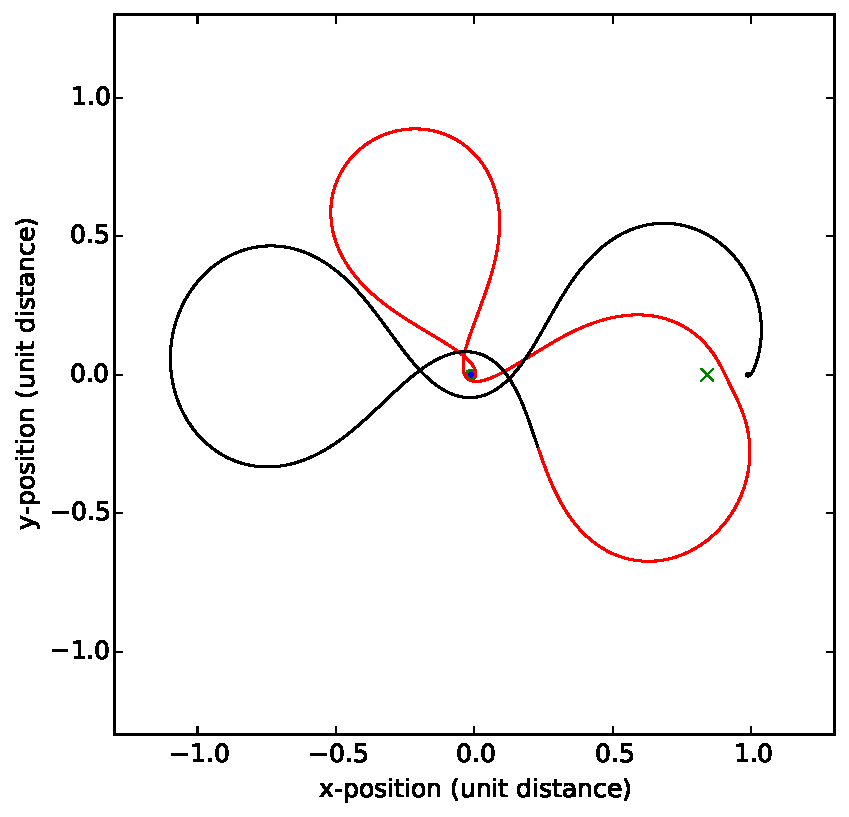
\includegraphics[scale=0.4]{fig/low-energy-short/_x-y_low_energy_short.pdf}    
        }
        \subbottom[Short LETO in $(\mathscr{X},\mathscr{Y})$, inertial system stationary on CM.]{
            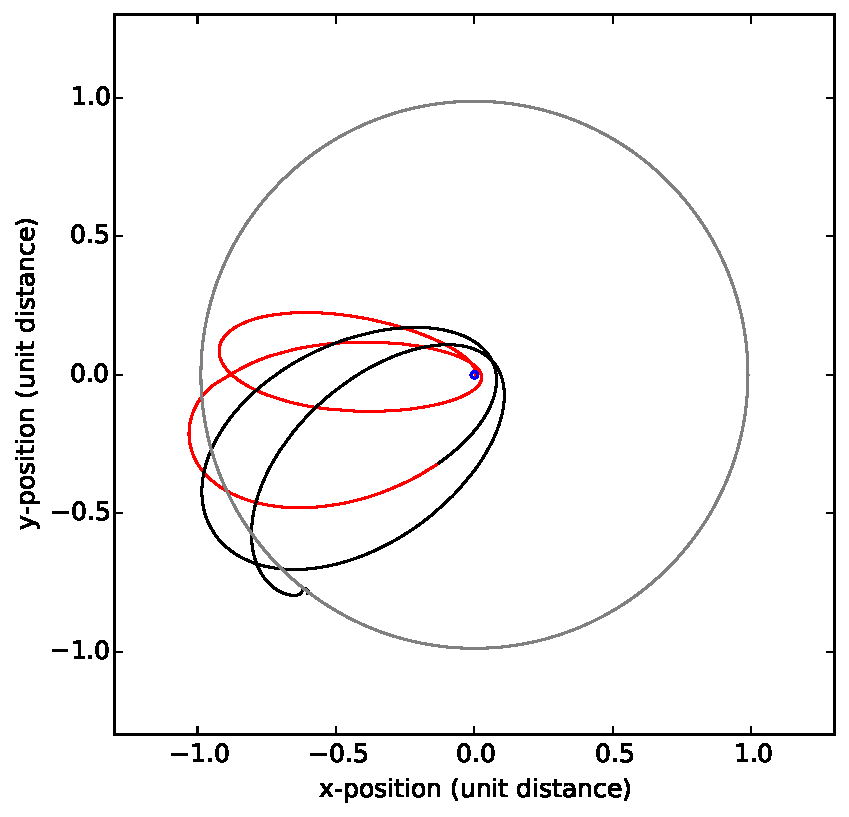
\includegraphics[scale=0.4]{fig/low-energy-short/X-Y_low_energy_short.pdf}
        }
        \caption{Position plots of short LETO. Earth in origin, moon orbit in grey, first half of trajectory is red, last half is black, green cross is first Lagrangepoint $L_1$}
        \label{fig:low_energy_short-position}
\end{figure}

\begin{figure}[ht!]
    \centering
        \subbottom[Exit from circular Earth parking orbit, $\SI{100}{\km}$ altitide]{
            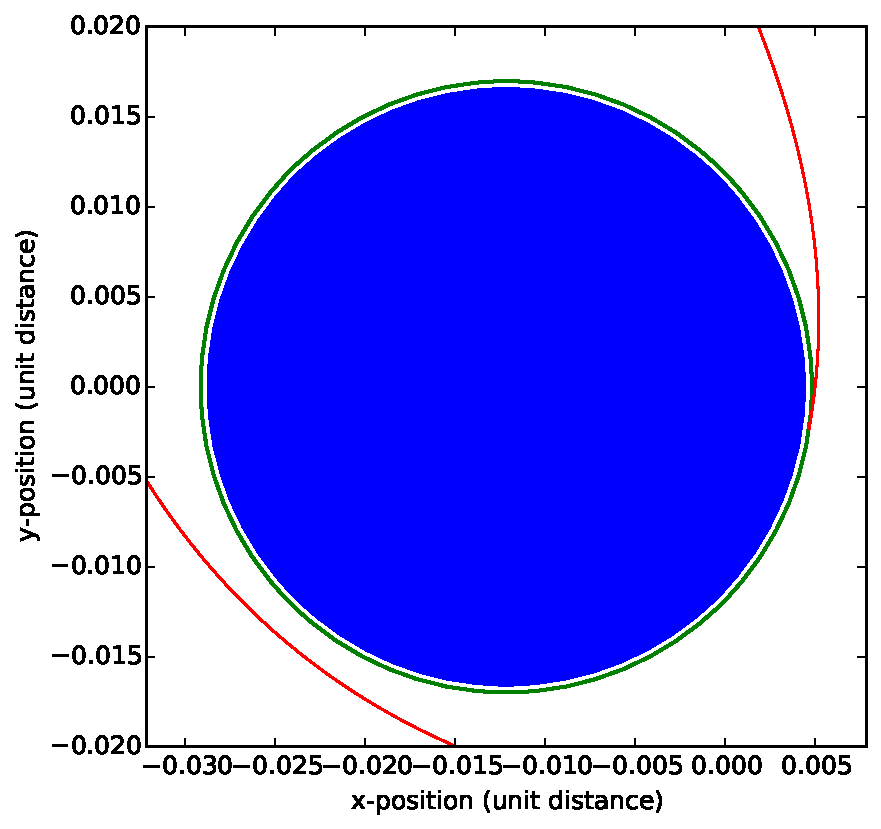
\includegraphics[scale=0.40]{fig/low-energy-short/earth_low_energy_short.pdf}    
        }
        \subbottom[Entry to circular Moon orbit, $\SI{100}{\km}$ altitude]{
            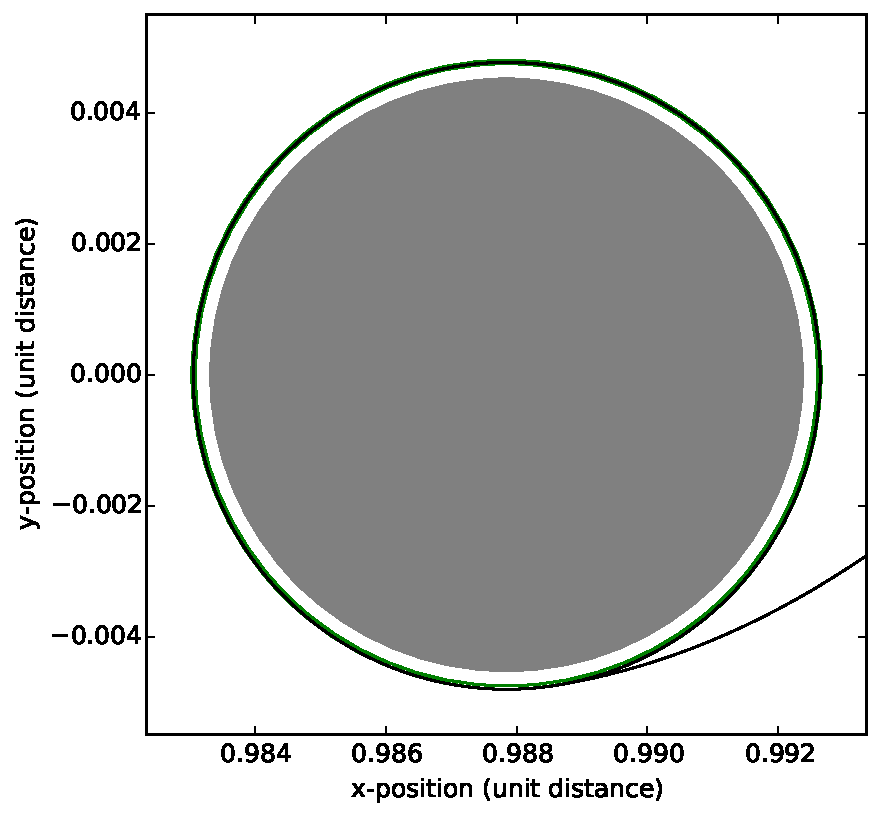
\includegraphics[scale=0.40]{fig/low-energy-short/moon_low_energy_short.pdf}
        }
        \caption{Exit- and entry orbits of short LETO. The green band around the moon is the altitude range of \SI{\pm 10}{\km} around \SI{100}{\km} that triggers a capture}
        \label{fig:low_energy_short-exit_entry}
\end{figure}

\begin{figure}[ht!]
    \centering
        \subbottom[Step size.]{
            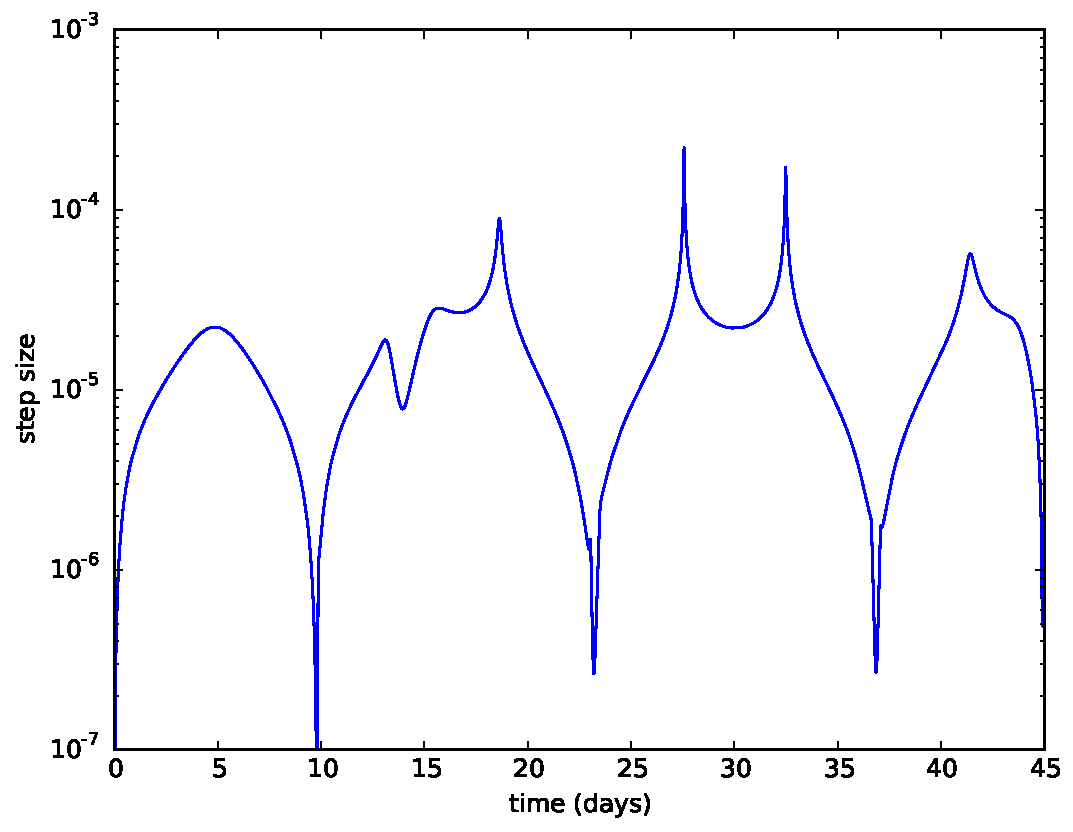
\includegraphics[scale=0.35]{fig/low-energy-short/step_low_energy_short.pdf}    
        }
        \subbottom[Error per step.]{
            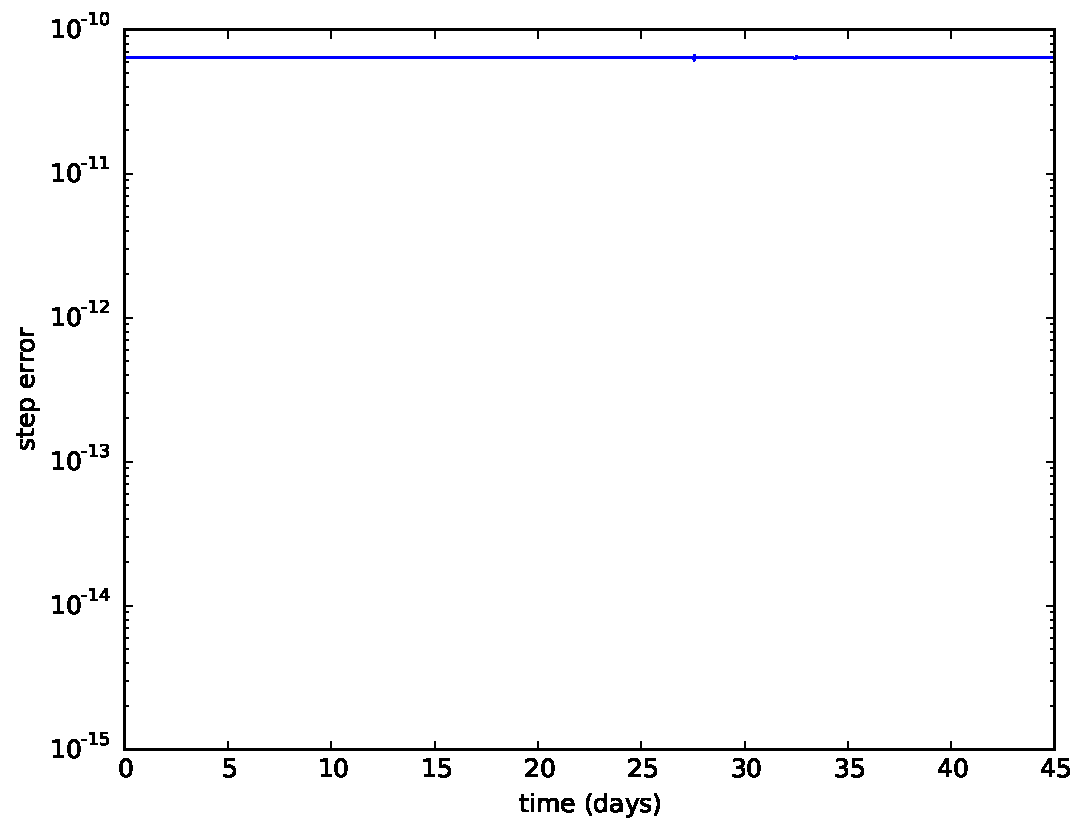
\includegraphics[scale=0.35]{fig/low-energy-short/err_low_energy_short.pdf}
        }
        \caption{Step size and error per step of simulated short LETO}
        \label{fig:low_energy_short-step_error}
\end{figure}

\begin{figure}[ht!]
\centering
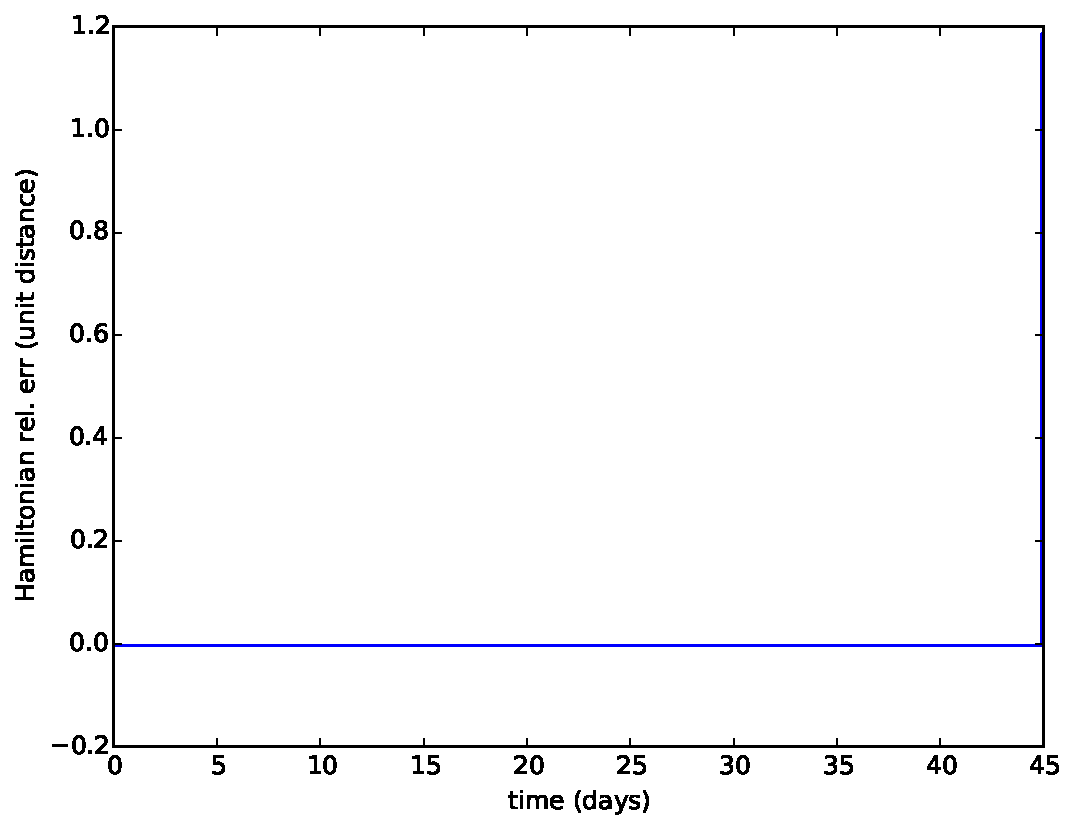
\includegraphics[scale=0.35]{fig/low-energy-short/H_low_energy_short.pdf}
\caption{Hamiltonian $H$ is conserved along the trajectory until $\Delta v_{\text{moon}}$ is applied, as expected}
\label{fig:low_energy_short-H}
\end{figure}

\clearpage
%\newpage
\vfill
%%%%%%%%%%%%%%%%%%%%%%%%%%%%%%%%%%%%%%%%%%%%%%%%%%%%%%%%%%%%%%%%%%%%%%%%%%%%%%
\subsection{Long LETO}
Listing \ref{lst:low_energy_long} show the lowest $\Delta v_{\text{total}}$ LETO trans-lunar injection 

%\begin{minipage}{\linewidth}
\begin{adjustwidth*}{0cm}{-0.4cm}
\begin{lstlisting}[caption={Long LETO. \texttt{pos} = angular difference with start angle (here $\theta=-3\pi/4$), \texttt{ang} = angle to velocity vector in Earth parking orbit, \texttt{burn} = $\Delta v_{\text{earth}}$, \texttt{(x0,y0,px0,py0)} are the initial conditions.},label=lst:low_energy_long]
# --------------------------------------------------------------------------
duration = 195/unit_time
pos      = 3.794182930145708
ang      = 0.023901745288554
burn     = 3.090702702702703/unit_vel
x0       = -0.025645129237870
y0       = -0.010311570301966
px0      = 6.539303578815582
py0      = -8.449205705334165
# --------------------------------------------------------------------------
# dV(earth-escape) = 3.090703 km/s
# dV(moon-capture) = 0.704113 km/s
# dV(total)        = 3.794815 km/s
# Flight-time      = 194.275487 days
# --------------------------------------------------------------------------
# Runtime = 0.98s
# Final position: 0.992404 0.001553
# Final impulse: 0.509302 -0.516927
# Final H: -2.730123
# Total runtime = 1.16s
# --------------------------------------------------------------------------
\end{lstlisting}
\end{adjustwidth*}
%\end{minipage}

See figure \ref{fig:low_energy_long-position} - \ref{fig:low_energy_long-H} for trajectory position-, entry/exit- and Hamiltonian plots.

\begin{figure}[ht!]
    \centering
        \subbottom[Long LETO in co-rotating $(x,y)$, Earth and Moon stationary.]{
            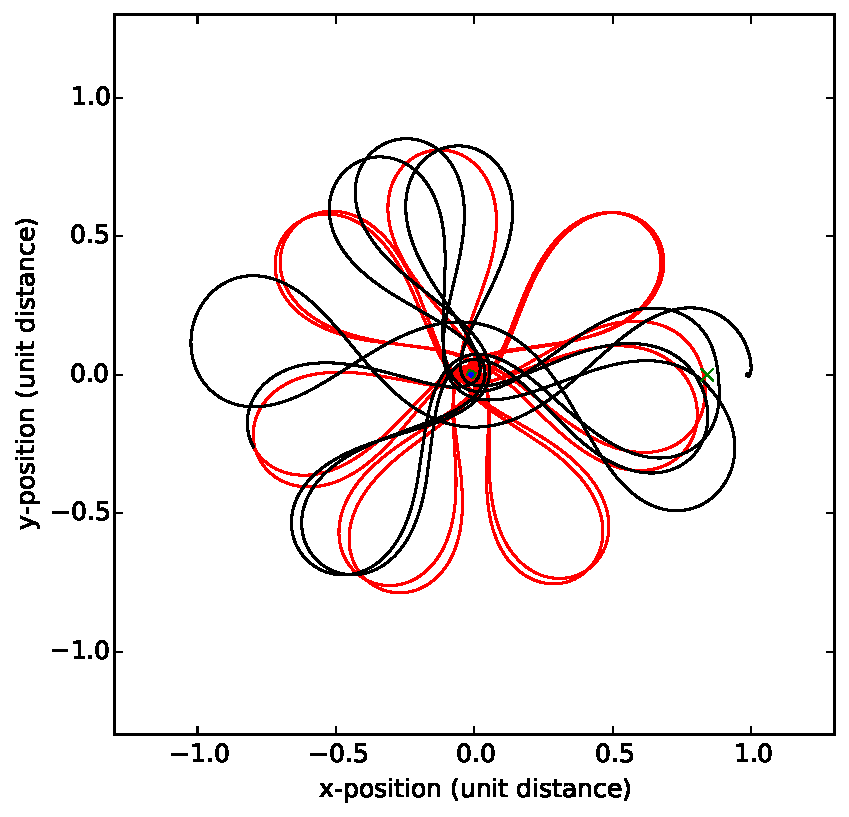
\includegraphics[scale=0.4]{fig/low-energy-long/_x-y_low_energy_long.pdf}    
        }
        \subbottom[Long LETO in $(\mathscr{X},\mathscr{Y})$, inertial system stationary on CM.]{
            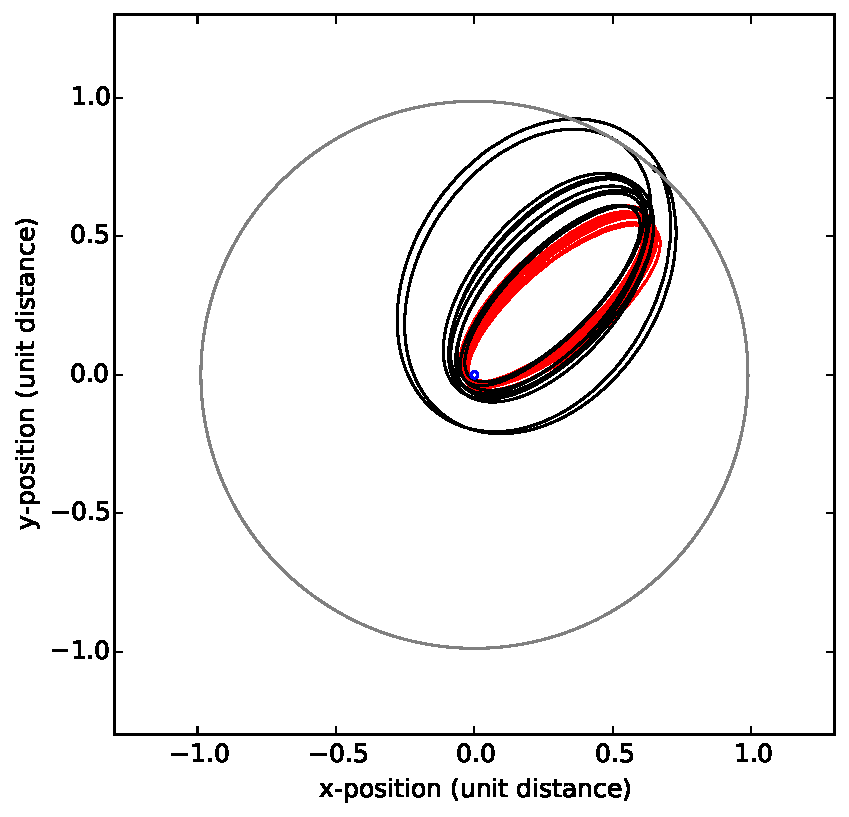
\includegraphics[scale=0.4]{fig/low-energy-long/X-Y_low_energy_long.pdf}
        }
        \caption{Position plots of long LETO. Earth in origin, moon orbit in grey, first half of trajectory is red, last half is black, green cross is first Lagrangepoint $L_1$}
        \label{fig:low_energy_long-position}
\end{figure}

\begin{figure}[ht!]
    \centering
        \subbottom[Exit from circular Earth parking orbit, $\SI{100}{\km}$ altitide]{
            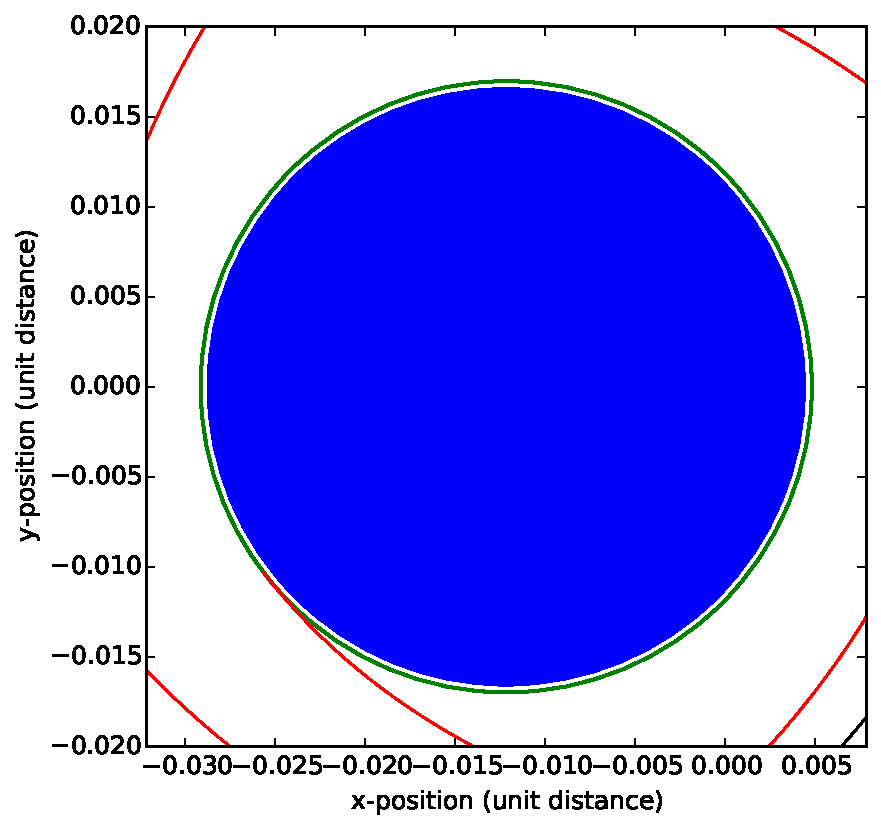
\includegraphics[scale=0.40]{fig/low-energy-long/earth_low_energy_long.pdf}    
        }
        \subbottom[Entry to circular Moon orbit, $\SI{100}{\km}$ altitude]{
            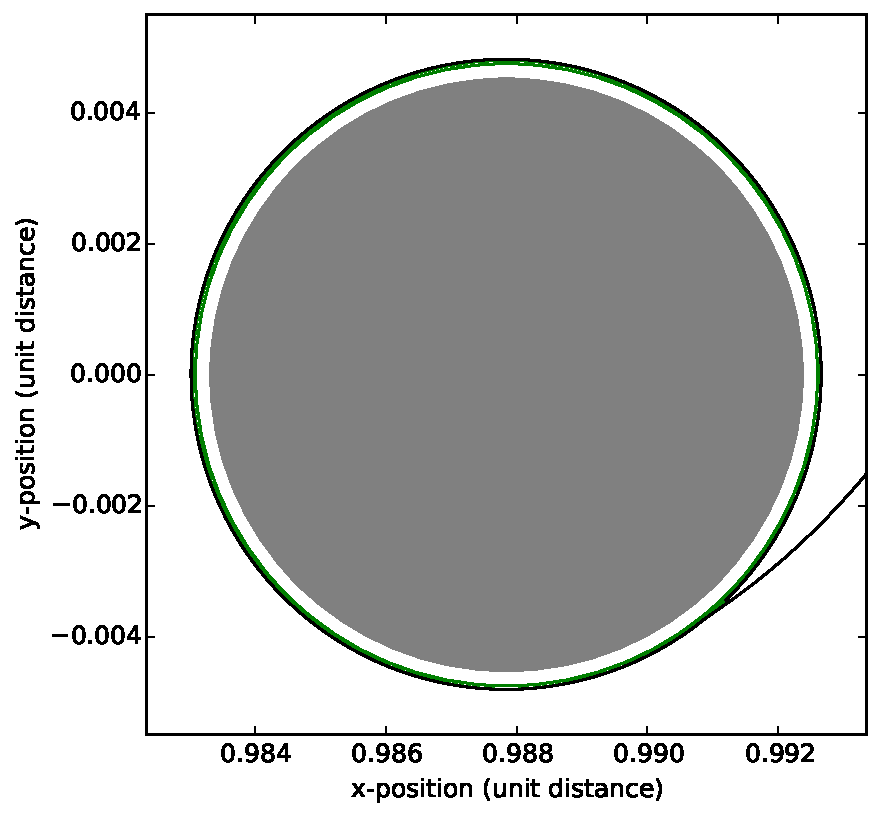
\includegraphics[scale=0.40]{fig/low-energy-long/moon_low_energy_long.pdf}
        }
        \caption{Exit- and entry orbits of long LETO. The green band around the moon is the altitude range of \SI{\pm 10}{\km} around \SI{100}{\km} that triggers a capture}
        \label{fig:low_energy_long-exit_entry}
\end{figure}

\begin{figure}[ht!]
    \centering
        \subbottom[Step size.]{
            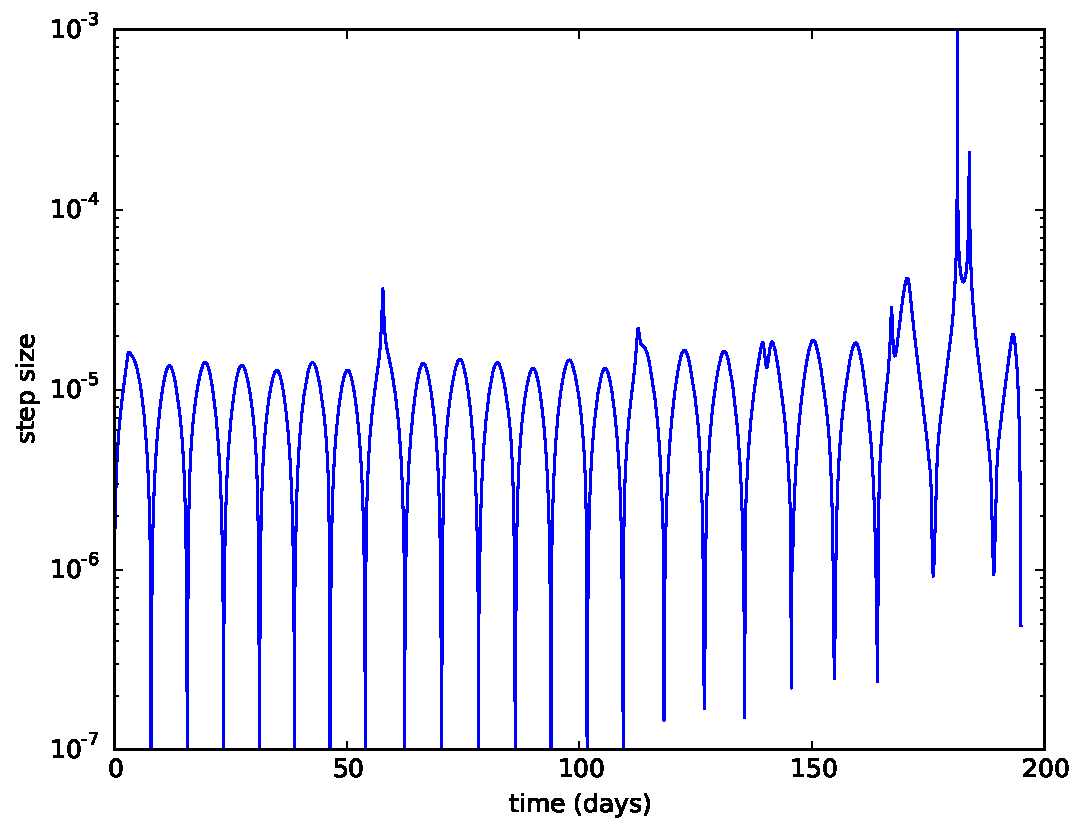
\includegraphics[scale=0.35]{fig/low-energy-long/step_low_energy_long.pdf}    
        }
        \subbottom[Error per step.]{
            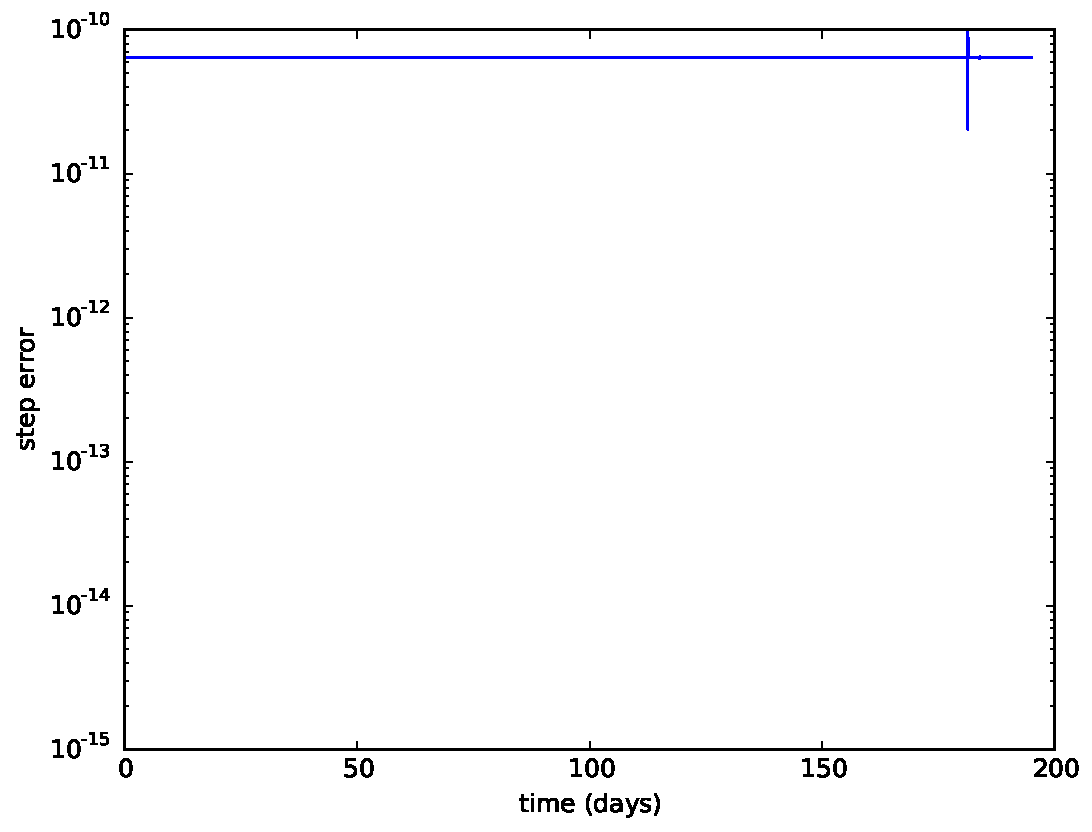
\includegraphics[scale=0.35]{fig/low-energy-long/err_low_energy_long.pdf}
        }
        \caption{Step size and error per step of simulated long LETO}
        \label{fig:low_energy_long-step_error}
\end{figure}

\vfill
\clearpage

\begin{figure}[ht!]
\centering
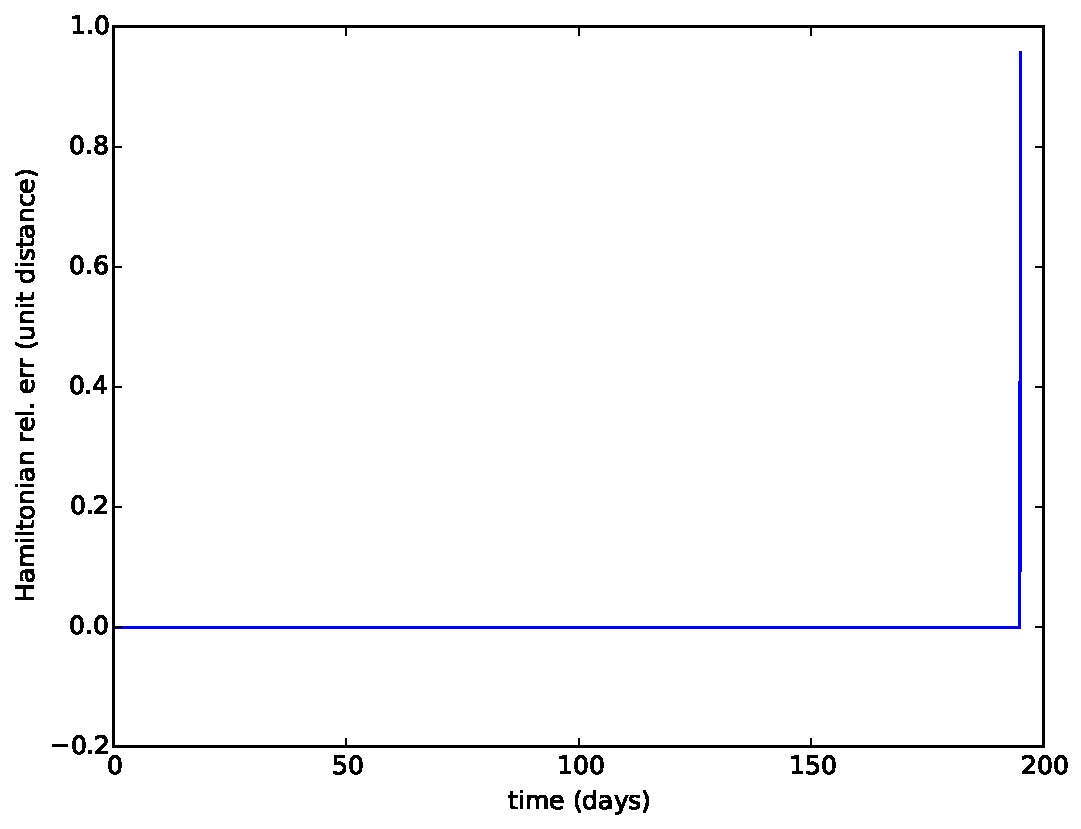
\includegraphics[scale=0.35]{fig/low-energy-long/H_low_energy_long.pdf}
\caption{Hamiltonian $H$ is conserved along the trajectory until $\Delta v_{\text{moon}}$ is applied, as expected}
\label{fig:low_energy_long-H}
\end{figure}


%%%%%%%%%%%%%%%%%%%%%%%%%%%%%%%%%%%%%%%%%%%%%%%%%%%%%%%%%%%%%%%%%%%%%%%%%%%%%%
\section{Results Summary and Discussion}
Table \ref{tab:results} summerizes the $\Delta v$ we found for the Hohmann, and the low-energy transfer orbts, short LETO and long LETO. In addition we've added a few more Hohmann (appendix \ref{app:more_hohmann}) to showcase the $Delta v$ vs. flight time dynamics and to compare with the Apollo missions. In early simulations, the brute force approach was good enough to find a good Hohmann transfer, but not good enough for low-energy. After some code optimization, parallelization and running sufficiently many simulations on multi-core processors yielded good resulsts even for low-energy transfers in the end.

\begin{itemize}
    \item The brute force method worked surpringsly well; we were able to find low-energy transfer orbits of lower $\Delta v$ than any of the two cited from literature.
    \item Results for the 3-day Hohmann are with 2.5\% of the Apollo $\Delta v$ and flight time, which adds to the credibility of our problem model and implementation.
    \item It would possibly be advantagous to go up to a symplectic 4.-5.th order Runge-Kutta method, but was not implemented due to time-constraints. However we do see that the error can be kept small around $10^{-9}$ within a reasonable runtime, which can somewhat justify staying in 2nd order methods. In other words, we would not necessarily find better results, just a bit lower runtime since we could take fewer steps with a 4th order method.
    \item In further investigations it would be interesting to include:
    \begin{enumerate}
        \item Patch together orbits in Lagrange points. This could be done by patching together brute forced trajectories from Earth to $L_1$ (integrated forwards) and $L_1$ to moon (integrated backwards).
        \item To from 2 to 3 dimensions.
        \item Include the gravitational force from the Sun. This allows us to explot the dynamics of the Sun-Earth-Moon system. For example deliberately approach the moon from the far side ($L_2$) \cite{Koon2001}.
        \item Exploit the dynamics of the Moon resonances as described in \cite{Topputo2005}.
    \end{enumerate}
\end{itemize}

\begin{table}
    \begin{tabular}{|l|l|l|l|l|}
    \hline
    Trajectory                    & Flight time             & $\Delta v_{\text{total}}$ (\scriptsize{km/s)} & $\Delta v_{\text{earth}}$ (\scriptsize{km/s)} & $\Delta v_{\text{moon}}$ (\scriptsize{km/s)} \\ \hline
    Minimum                       & N/A                     & 3.721                     & 3.099                     & 0.622                    \\ \hline
    Long LETO                     & 194 days  & 3.795                     & 3.091                     & 0.704                    \\ \hline
    Belbruno-Miller               & 3 months                & 3.838                     & 3.187                     & 0.651                    \\ \hline
    Topputo                       & 8 months                & 3.895                     & 3.265                     & 0.630                    \\ \hline
    Short LETO                    & 41 days                 & 3.896                     & 3.127                     & 0.769                    \\ \hline
    Hohmann - long (sim)   & 4.3 days                & 3.912                     & 3.111                     & 0.801                    \\ \hline
    Hohmann - (model)      & 5.0 days                & 3.946                     & 3.144                     & 0.802                    \\ \hline
    Hohmann - medium (sim) & 3.00 days               & 4.015                     & 3.136                     & 0.880                    \\ \hline
    Apollo (Hohman)      & 3.05 days               & 4.115                     & 3.048                     & 1.067                    \\ \hline
    Hohmann - short (sim)  & 1.00 days               & 6.823                     & 3.809                     & 3.014                    \\ \hline
\end{tabular}
\caption{Summerized flight time and $\Delta v$ for various trajectories, sorted by $\Delta v_{\text{total}}$. Belbruno and Topputo from \cite{Juul2008} are for orbits going from \SI{167}{\km} Earth parking to \SI{100}{\km} circular moon orbit. Apollo mission data form \cite{NASA1966} \cite{apollo-timeline}.}
\label{tab:results}
\end{table}

%$\si{\km\per\s}$